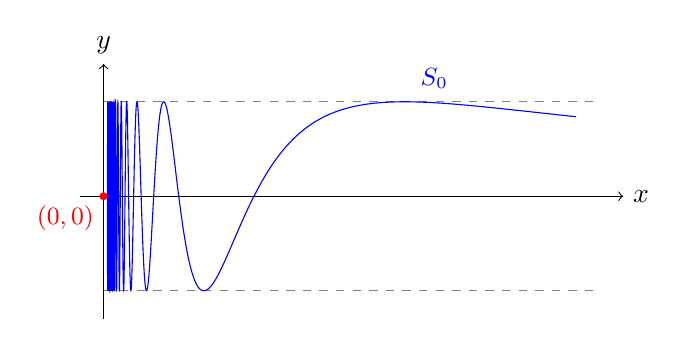
\begin{tikzpicture}[xscale=6, yscale=1.2]
  \draw[->] (-0.05,0) -- (1.1,0) node[right] {$x$};
  \draw[->] (0,-1.3) -- (0,1.4) node[above] {$y$};
  \draw[dashed, gray] (0,1) -- (1.05,1);
  \draw[dashed, gray] (0,-1) -- (1.05,-1);
  \draw[blue, thin, variable=\t, domain=1:120, samples=2400] plot ({1/\t}, {sin(deg(\t))});
  \fill[red] (0,0) circle (0.25pt and 1.2pt);
  \node[red, below left] at (0,0) {\small $(0,0)$};
  \node[blue] at (0.7,1.25) {\small $S_0$};
\end{tikzpicture}
